% pi-402: Paying for Inference with Sats
% LaTeX Beamer Presentation
% Author: Laolu Osuntokun

\documentclass[aspectratio=169,11pt]{beamer}

% ============================================================================
% THEME SETUP - Lightning Labs modern style (shared with the PQ / format
% modeling talks).
% ============================================================================

\usetheme{default}
\usecolortheme{default}

\definecolor{llpurple}{HTML}{7B2FF2}
\definecolor{llorange}{HTML}{F5A623}
\definecolor{llyellowgreen}{HTML}{CDDC39}
\definecolor{llcyan}{HTML}{4DD0B8}
\definecolor{lllightblue}{HTML}{64B5F6}
\definecolor{llred}{HTML}{E0533D}

\definecolor{llblack}{HTML}{0A0A0A}
\definecolor{llwhite}{HTML}{FFFFFF}
\definecolor{llcardbg}{HTML}{F0F0F0}
\definecolor{llcodebg}{HTML}{F6F4FB}
\definecolor{lldarktext}{HTML}{1A1A1A}
\definecolor{llgraytext}{HTML}{555555}
\definecolor{llgraylight}{HTML}{999999}

\setbeamercolor{background canvas}{bg=llwhite}
\setbeamercolor{normal text}{fg=lldarktext}
\setbeamercolor{title}{fg=llwhite}
\setbeamercolor{frametitle}{fg=lldarktext}
\setbeamercolor{item}{fg=llpurple}
\setbeamercolor{itemize item}{fg=llpurple}
\setbeamercolor{itemize subitem}{fg=llcyan}
\setbeamercolor{enumerate item}{fg=llpurple}
\setbeamercolor{block title}{fg=llwhite,bg=llpurple}
\setbeamercolor{block body}{fg=lldarktext,bg=llcardbg}
\setbeamercolor{alerted text}{fg=llorange}
\setbeamercolor{structure}{fg=llpurple}

\setbeamerfont{title}{size=\Huge,series=\bfseries}
\setbeamerfont{frametitle}{size=\Large,series=\bfseries}

\setbeamertemplate{navigation symbols}{}
\setbeamertemplate{footline}{}
\setbeamertemplate{frametitle}{}

\setbeamertemplate{itemize item}{\textcolor{llpurple}{\raisebox{0.2ex}{\tiny$\blacksquare$}}}
\setbeamertemplate{itemize subitem}{\textcolor{llcyan}{\raisebox{0.1ex}{\small--}}}

% ============================================================================
% PACKAGES
% ============================================================================

\usepackage[utf8]{inputenc}
\usepackage[T1]{fontenc}
\usepackage{lmodern}
\renewcommand{\familydefault}{\sfdefault}
\usepackage{tikz}
\usetikzlibrary{shapes,arrows,positioning,fit,calc,backgrounds,
  decorations.pathreplacing,arrows.meta}
\usepackage{graphicx}
\usepackage{hyperref}
\usepackage{amssymb}
\usepackage{tabularx}
\usepackage{array}
\usepackage{listings}
\usepackage{booktabs}

\DeclareUnicodeCharacter{00A7}{\S}
\DeclareUnicodeCharacter{2192}{$\rightarrow$}
\DeclareUnicodeCharacter{2190}{$\leftarrow$}
\DeclareUnicodeCharacter{2194}{$\leftrightarrow$}
\DeclareUnicodeCharacter{2264}{$\leq$}
\DeclareUnicodeCharacter{2265}{$\geq$}
\DeclareUnicodeCharacter{00D7}{$\times$}
\DeclareUnicodeCharacter{2013}{--}
\DeclareUnicodeCharacter{2014}{---}
\DeclareUnicodeCharacter{2018}{`}
\DeclareUnicodeCharacter{2019}{'}
\DeclareUnicodeCharacter{201C}{``}
\DeclareUnicodeCharacter{201D}{''}
\DeclareUnicodeCharacter{2026}{\ldots}
\DeclareUnicodeCharacter{25A0}{$\blacksquare$}
\DeclareUnicodeCharacter{2248}{$\approx$}
\DeclareUnicodeCharacter{00B7}{$\cdot$}
\DeclareUnicodeCharacter{26A1}{$\lightning$}

% ============================================================================
% LISTING STYLES
% ============================================================================

\lstdefinestyle{spec}{
  language={},
  basicstyle=\ttfamily\scriptsize\color{lldarktext},
  keywordstyle=\color{lldarktext},
  commentstyle=\color{lldarktext},
  backgroundcolor=\color{llcardbg},
  frame=leftline,
  framerule=2pt,
  rulecolor=\color{llorange},
  framesep=6pt,
  xleftmargin=10pt,
  breaklines=true,
  columns=fullflexible,
}

\lstdefinestyle{code}{
  language={},
  basicstyle=\ttfamily\fontsize{7.6}{9}\selectfont\color{lldarktext},
  keywordstyle=\color{llpurple}\bfseries,
  commentstyle=\color{llgraytext}\itshape,
  backgroundcolor=\color{llcodebg},
  frame=leftline,
  framerule=2pt,
  rulecolor=\color{llpurple},
  framesep=6pt,
  xleftmargin=10pt,
  showstringspaces=false,
  breaklines=true,
  columns=fullflexible,
  keepspaces=true,
}

% ============================================================================
% CUSTOM TIKZ / HELPER COMMANDS
% ============================================================================

\newcommand{\drawDecorativeSquares}{%
  \begin{tikzpicture}[remember picture, overlay]
    \fill[llyellowgreen] ([shift={(-3.2cm,-0.6cm)}]current page.north east)
      rectangle ++(0.55cm,0.55cm);
    \fill[llcyan] ([shift={(-2.4cm,-0.6cm)}]current page.north east)
      rectangle ++(0.55cm,0.55cm);
    \fill[llpurple] ([shift={(-1.6cm,-0.6cm)}]current page.north east)
      rectangle ++(0.55cm,0.55cm);
    \fill[llcyan] ([shift={(-1.8cm,-1.4cm)}]current page.north east)
      rectangle ++(0.45cm,0.45cm);
    \fill[llorange] ([shift={(-0.9cm,-1.7cm)}]current page.north east)
      rectangle ++(0.6cm,0.6cm);
    \fill[llorange] ([shift={(-0.5cm,-2.8cm)}]current page.north east)
      rectangle ++(0.5cm,0.5cm);
    \fill[llpurple] ([shift={(-0.4cm,-3.6cm)}]current page.north east)
      rectangle ++(0.5cm,0.5cm);
    \fill[lllightblue] ([shift={(-0.7cm,-4.5cm)}]current page.north east)
      rectangle ++(0.5cm,0.5cm);
  \end{tikzpicture}%
}

\newcommand{\sectiontitle}[1]{%
  \vspace{-0.10cm}%
  \begin{tikzpicture}
    \node[anchor=west, font=\Large\bfseries, text=lldarktext] (title) at (0,0) {#1};
    \fill[llpurple] ([yshift=-4pt]title.south west)
      rectangle ([yshift=-7pt,xshift=2.8cm]title.south west);
  \end{tikzpicture}%
  \vspace{0.02cm}%
}

\newcommand{\slidefooter}{%
  \begin{tikzpicture}[remember picture, overlay]
    \node[anchor=south west, font=\tiny\color{llgraylight}]
      at ([shift={(0.5cm,0.16cm)}]current page.south west)
      {pi-402: Paying for Inference with Sats --- Lightning Labs};
    \node[anchor=south east, font=\tiny\color{llgraylight}]
      at ([shift={(-0.5cm,0.16cm)}]current page.south east)
      {\insertframenumber/\inserttotalframenumber};
  \end{tikzpicture}%
}

% A colored chip for inline labels.
\newcommand{\chip}[1]{%
  \tikz[baseline=(b.base)]{\node[fill=llpurple, text=white,
    font=\footnotesize\bfseries, inner sep=3pt, rounded corners=1pt] (b) {#1};}%
}
\newcommand{\ochip}[1]{%
  \tikz[baseline=(b.base)]{\node[fill=llorange, text=white,
    font=\footnotesize\bfseries, inner sep=3pt, rounded corners=1pt] (b) {#1};}%
}

% Labeled mini-row.
\newcommand{\frow}[2]{{\scriptsize\textbf{\textcolor{llpurple}{#1}} #2}\par\vspace{2pt}}

% A big stat block: number + caption.
\newcommand{\statblock}[3]{%
  \begin{minipage}[t]{#1}
    \centering
    {\fontsize{20}{22}\selectfont\bfseries\color{llpurple}#2}\\[2pt]
    {\fontsize{7.4}{8.6}\selectfont\color{llgraytext}#3}
  \end{minipage}%
}

% ============================================================================
% DOCUMENT
% ============================================================================

\begin{document}

% ----------------------------------------------------------------------------
% SLIDE 1: TITLE
% ----------------------------------------------------------------------------
\begin{frame}[plain]
  \begin{tikzpicture}[remember picture, overlay]
    \fill[llblack] (current page.south west) rectangle (current page.north east);
  \end{tikzpicture}
  \drawDecorativeSquares
  \begin{tikzpicture}[remember picture, overlay]
    \node[anchor=north west, text=white, font=\small\bfseries]
      at ([shift={(0.8cm,-0.6cm)}]current page.north west)
      {$\boldsymbol{\diamond}$\kern2pt Lightning Labs};
    \node[anchor=north west, text=white, font=\fontsize{40}{46}\selectfont\bfseries]
      at ([shift={(1.2cm,-1.9cm)}]current page.north west)
      {\begin{tabular}{@{}l@{}}pi-402\end{tabular}};
    \node[anchor=north west, text=llyellowgreen, font=\Large\bfseries]
      at ([shift={(1.2cm,-3.3cm)}]current page.north west)
      {Paying for Kimi K3 with sats};
    \node[anchor=north west, text=llcyan, font=\large, text width=11.5cm]
      at ([shift={(1.2cm,-4.7cm)}]current page.north west)
      {The strongest open-weights model on earth, metered by the token and
       settled over Lightning. No account, no API key, no credit card.};
    \node[anchor=south west, text=llgraylight, font=\tiny]
      at ([shift={(0.8cm,0.4cm)}]current page.south west)
      {Olaoluwa Osuntokun --- Lightning Labs};
  \end{tikzpicture}
\end{frame}

% ----------------------------------------------------------------------------
% SLIDE 2: WHY THIS MATTERS
% ----------------------------------------------------------------------------
\begin{frame}[plain]
  \sectiontitle{The Best Open Model Is Behind a Credit Card}
  \vspace{0.12cm}

  {\footnotesize Moonshot released the Kimi K3 weights on \textbf{2026-07-27},
  the \#1 open model on Artificial Analysis. Anyone may download it, and almost
  nobody can run it: it wants a rack of GB300s. So ``open weights'' means
  ``open to whoever will sell you inference,'' and that gate isn't the weights,
  it's the payment rail.}

  \vspace{0.16cm}
  \begin{center}
    \statblock{2.3cm}{2.8T}{parameters}\hfill
    \statblock{2.3cm}{16/896}{experts active}\hfill
    \statblock{2.3cm}{1M}{token context}\hfill
    \statblock{2.3cm}{vision}{natively multimodal}\hfill
    \statblock{2.3cm}{1.5\,TB}{the download}
  \end{center}

  \vspace{0.3cm}
  \begin{minipage}[t]{0.475\textwidth}
    {\footnotesize\textbf{\textcolor{llred}{What the card rail costs you}}}\par
    \vspace{3pt}
    {\fontsize{7.6}{9.4}\selectfont
    An account and a fraud check, upstream of the first token. Declines by
    geography and by bank. No card for an autonomous agent, and handing it
    yours makes it you. Card economics can't clear a \$0.01 request.}
  \end{minipage}\hfill
  \begin{minipage}[t]{0.475\textwidth}
    {\footnotesize\textbf{\textcolor{llcyan}{What sats give you instead}}}\par
    \vspace{3pt}
    {\fontsize{7.6}{9.4}\selectfont
    The payment \emph{is} the credential: no identity to establish, leak, or
    revoke. The buyer's country is not an input. An agent holds a wallet, and
    the balance you fund is the blast radius. Sub-cent amounts clear.}
  \end{minipage}

  \vspace{0.26cm}
  {\footnotesize The scarce thing was never the model, it's
  \textbf{\textcolor{llpurple}{permission to pay for it}}.}

  \slidefooter
\end{frame}

% ----------------------------------------------------------------------------
% SLIDE 3: WHAT WE BUILT
% ----------------------------------------------------------------------------
\begin{frame}[plain]
  \sectiontitle{What We Built}
  \vspace{0.1cm}

  {\footnotesize A coding agent that pays per call. The buyer is a Pi
  extension, the seller is an aperture proxy holding the model credential, and
  the two meet over L402.}

  \vspace{0.3cm}
  \begin{center}
  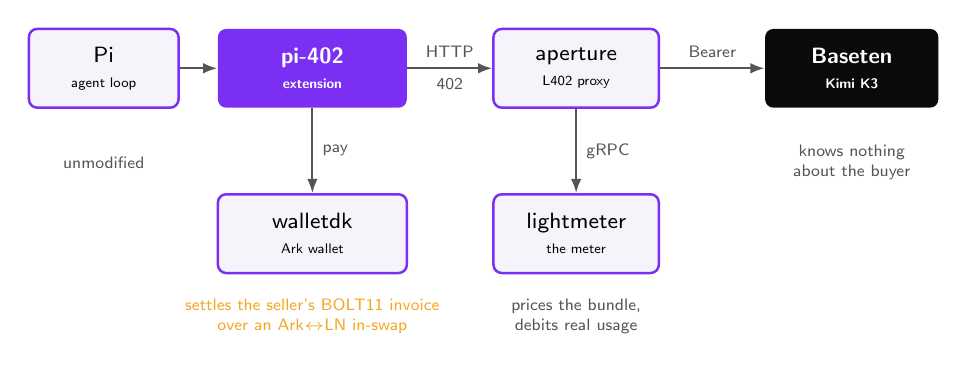
\begin{tikzpicture}[
    box/.style={rectangle, rounded corners=3pt, draw=llpurple, line width=0.9pt,
      fill=llcodebg, align=center, font=\fontsize{7.6}{9}\selectfont,
      minimum height=1.0cm, inner sep=5pt},
    dark/.style={rectangle, rounded corners=3pt, fill=llpurple, text=white,
      align=center, font=\fontsize{7.6}{9}\selectfont\bfseries,
      minimum height=1.0cm, inner sep=5pt},
    up/.style={rectangle, rounded corners=3pt, fill=llblack, text=white,
      align=center, font=\fontsize{7.6}{9}\selectfont\bfseries,
      minimum height=1.0cm, inner sep=5pt},
    a/.style={-{Latex[length=1.8mm]}, llgraytext, line width=0.8pt},
    lbl/.style={font=\fontsize{6.2}{7.2}\selectfont, text=llgraytext, align=center},
  ]
    \node[box, minimum width=1.9cm] (pi) at (-5.5,0) {Pi\\{\tiny agent loop}};
    \node[dark, minimum width=2.4cm] (ext) at (-2.85,0) {pi-402\\{\tiny extension}};
    \node[box, minimum width=2.1cm] (ap) at (0.5,0) {aperture\\{\tiny L402 proxy}};
    \node[box, minimum width=2.1cm] (lm) at (0.5,-2.1) {lightmeter\\{\tiny the meter}};
    \node[up, minimum width=2.2cm] (bt) at (4.0,0) {Baseten\\{\tiny Kimi K3}};
    \node[box, minimum width=2.4cm] (w) at (-2.85,-2.1) {walletdk\\{\tiny Ark wallet}};

    \draw[a] (pi) -- (ext);
    \draw[a] (ext) -- node[lbl, above]{HTTP} node[lbl, below]{402} (ap);
    \draw[a] (ap) -- node[lbl, above]{Bearer} (bt);
    \draw[a] (ext) -- node[lbl, right]{pay} (w);
    \draw[a] (ap) -- node[lbl, right]{gRPC} (lm);

    \node[lbl] at (-5.5,-1.2) {unmodified};
    \node[lbl] at (4.0,-1.2) {knows nothing\\about the buyer};
    \node[lbl, text=llorange, align=center] at (-2.85,-3.15)
      {settles the seller's BOLT11 invoice\\over an Ark$\leftrightarrow$LN in-swap};
    \node[lbl, align=center] at (0.5,-3.15)
      {prices the bundle,\\debits real usage};
  \end{tikzpicture}
  \end{center}

  \vspace{0.25cm}
  {\footnotesize Two properties fall out of this shape.
  \textbf{\textcolor{llpurple}{Pi core is never modified}}, because every hook
  is a documented extension point. And
  \textbf{\textcolor{llpurple}{no API key ever reaches the buyer}}, because
  aperture injects the model credential server-side. The buyer holds sats; the
  seller holds the key.}

  \slidefooter
\end{frame}

% ----------------------------------------------------------------------------
% SLIDE 4: WHY PI + THE EXTENSION SURFACE
% ----------------------------------------------------------------------------
\begin{frame}[plain]
  \sectiontitle{Why Pi: Payment Lives Under the Model Call}
  \vspace{0.08cm}

  {\footnotesize Payment has to sit on the \emph{transport}, beneath the model
  call. That rules out most agents: if one owns its HTTP client and won't let
  you replace it, there's nowhere to put a payment loop short of forking it.
  Pi's \texttt{registerProvider} takes a \texttt{streamSimple} that builds its
  own client, so we hand it a \texttt{fetch} that knows how to pay.}

  \vspace{0.18cm}
  \begin{center}
  {\scriptsize
  \renewcommand{\arraystretch}{1.2}
  \begin{tabularx}{0.97\textwidth}{@{}l l X@{}}
    \textbf{What a payment layer needs} & \textbf{Pi hook} & \textbf{How we use it}\\
    \midrule
    A paying transport &
      \texttt{registerProvider} &
      \texttt{streamSimple} builds an OpenAI client whose \texttt{fetch} is
      \texttt{payingFetch}\\
    Point at the proxy, declare the model &
      provider config &
      \texttt{baseUrl} is the L402 proxy; \texttt{models:[\ldots]} declares
      \texttt{kimi-k3}\\
    Hold a wallet for the session &
      \texttt{on("session\_start")} &
      load and unlock the walletdk wallet once, then reuse it\\
    Fund and inspect, out of band &
      \texttt{registerCommand} &
      \texttt{/wallet} \texttt{/deposit} \texttt{/balance} \texttt{/receipts}\\
    Surface a declined payment &
      provider \texttt{error} event &
      budget rejections reach the user as a normal stream error\\
    \bottomrule
  \end{tabularx}}
  \end{center}

  \vspace{0.25cm}
  {\footnotesize Paid inference, \textbf{no change to Pi}, and
  \textbf{\textcolor{llpurple}{the agent core never learns money exists}}.}

  \slidefooter
\end{frame}

% ----------------------------------------------------------------------------
% SLIDE 5: L402 + THE BUYER LOOP
% ----------------------------------------------------------------------------
\begin{frame}[plain]
  \sectiontitle{L402: Two Primitives, One Loop}
  \vspace{0.08cm}

  {\footnotesize A macaroon (attenuatable, offline-verifiable authorization)
  and a payment preimage (atomic proof of settlement). The macaroon's
  identifier commits to a payment hash $H$; paying the invoice for $H$ reveals
  $r$ with $\mathrm{sha256}(r) = H$; the client presents \texttt{macaroon:r}.
  So \textbf{a valid credential cannot exist without settlement}, and
  settlement reveals exactly the secret that validates it.}

  \vspace{0.2cm}
  \begin{center}
  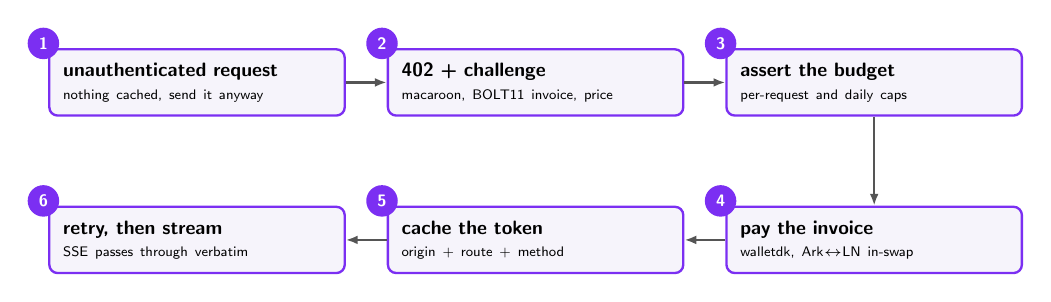
\begin{tikzpicture}[
    s/.style={rectangle, rounded corners=3pt, draw=llpurple, line width=0.85pt,
      fill=llcodebg, align=left, font=\fontsize{6.9}{8.1}\selectfont,
      minimum height=0.8cm, text width=3.4cm, inner sep=5pt},
    n/.style={circle, fill=llpurple, text=white,
      font=\fontsize{6.2}{7}\selectfont\bfseries, inner sep=1.5pt,
      minimum size=0.40cm},
    a/.style={-{Latex[length=1.5mm]}, llgraytext, line width=0.8pt},
  ]
    \node[s] (s1) at (-3.95,1.15) {\textbf{unauthenticated request}\\
      {\tiny nothing cached, send it anyway}};
    \node[s] (s2) at (0.35,1.15) {\textbf{402 + challenge}\\
      {\tiny macaroon, BOLT11 invoice, price}};
    \node[s] (s3) at (4.65,1.15) {\textbf{assert the budget}\\
      {\tiny per-request and daily caps}};
    \node[s] (s4) at (4.65,-0.85) {\textbf{pay the invoice}\\
      {\tiny walletdk, Ark$\leftrightarrow$LN in-swap}};
    \node[s] (s5) at (0.35,-0.85) {\textbf{cache the token}\\
      {\tiny origin + route + method}};
    \node[s] (s6) at (-3.95,-0.85) {\textbf{retry, then stream}\\
      {\tiny SSE passes through verbatim}};

    \node[n] at ([shift={(-0.06,0.06)}]s1.north west) {1};
    \node[n] at ([shift={(-0.06,0.06)}]s2.north west) {2};
    \node[n] at ([shift={(-0.06,0.06)}]s3.north west) {3};
    \node[n] at ([shift={(-0.06,0.06)}]s4.north west) {4};
    \node[n] at ([shift={(-0.06,0.06)}]s5.north west) {5};
    \node[n] at ([shift={(-0.06,0.06)}]s6.north west) {6};

    \draw[a] (s1) -- (s2);
    \draw[a] (s2) -- (s3);
    \draw[a] (s3) -- (s4);
    \draw[a] (s4) -- (s5);
    \draw[a] (s5) -- (s6);
  \end{tikzpicture}
  \end{center}

  \vspace{0.18cm}
  {\footnotesize
  \frow{Bootstrapping is free}{Step 1 costs nothing: the challenge and invoice
    are handed out unauthenticated, and \texttt{/deposit} never touches a
    model. A funded wallet is the only precondition.}
  \frow{An Ark wallet, not a node}{No channels, no inbound liquidity, nothing
    kept online. Fund a boarding address; an in-swap turns a VTXO into a
    Lightning payment.}}

  \slidefooter
\end{frame}

% ----------------------------------------------------------------------------
% SLIDE 6: METERING, THE EXISTING IMPLEMENTATION
% ----------------------------------------------------------------------------
\begin{frame}[plain]
  \sectiontitle{Metering Aperture: Four Call-Outs, Shipping Today}
  \vspace{0.06cm}

  {\footnotesize Aperture mints challenges, verifies credentials, and forwards.
  What it can't do is charge by the token, since it has no idea what an LLM is.
  So we didn't teach it: a separate daemon implements the
  \texttt{pricesrpc.Prices} gRPC service and owns all cost analysis.}

  \vspace{0.14cm}
  \begin{center}
  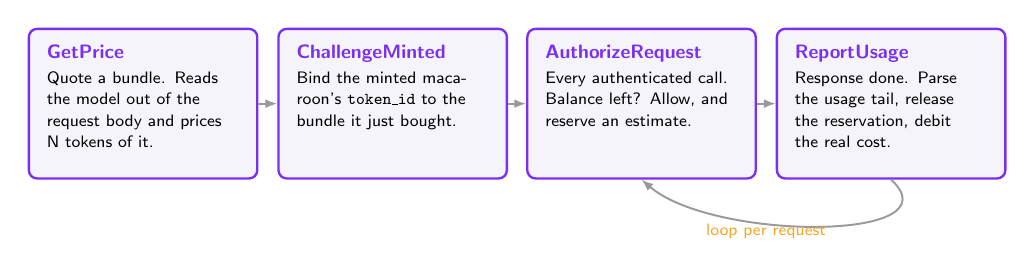
\begin{tikzpicture}[
    r/.style={rectangle, rounded corners=3pt, draw=llpurple, line width=0.85pt,
      fill=llcodebg, align=left, minimum height=1.9cm, text width=2.55cm,
      inner sep=5pt},
    hd/.style={font=\fontsize{7.2}{8.4}\selectfont\bfseries, text=llpurple},
    bd/.style={font=\fontsize{6.5}{7.7}\selectfont, text width=2.32cm},
    a/.style={-{Latex[length=1.5mm]}, llgraylight, line width=0.7pt},
  ]
    \node[r] (a1) at (-4.75,0) {};
    \node[r] (a2) at (-1.58,0) {};
    \node[r] (a3) at (1.58,0) {};
    \node[r] (a4) at (4.75,0) {};

    \node[anchor=north west, hd] at ([shift={(0.12,-0.10)}]a1.north west) {GetPrice};
    \node[anchor=north west, bd] at ([shift={(0.12,-0.44)}]a1.north west)
      {Quote a bundle. Reads the model out of the request body and prices N
       tokens of it.};

    \node[anchor=north west, hd] at ([shift={(0.12,-0.10)}]a2.north west) {ChallengeMinted};
    \node[anchor=north west, bd] at ([shift={(0.12,-0.44)}]a2.north west)
      {Bind the minted macaroon's \texttt{token\_id} to the bundle it just
       bought.};

    \node[anchor=north west, hd] at ([shift={(0.12,-0.10)}]a3.north west) {AuthorizeRequest};
    \node[anchor=north west, bd] at ([shift={(0.12,-0.44)}]a3.north west)
      {Every authenticated call. Balance left? Allow, and reserve an
       estimate.};

    \node[anchor=north west, hd] at ([shift={(0.12,-0.10)}]a4.north west) {ReportUsage};
    \node[anchor=north west, bd] at ([shift={(0.12,-0.44)}]a4.north west)
      {Response done. Parse the usage tail, release the reservation, debit
       the real cost.};

    \draw[a] (a1) -- (a2);
    \draw[a] (a2) -- (a3);
    \draw[a] (a3) -- (a4);
    \draw[a] (a4.south) .. controls (5.6,-1.75) and (2.5,-1.75) .. (a3.south);
    \node[font=\fontsize{6.0}{7}\selectfont, text=llorange] at (3.16,-1.62)
      {loop per request};
  \end{tikzpicture}
  \end{center}

  \vspace{0.1cm}
  {\footnotesize
  \frow{The move that makes it work}{\texttt{AuthorizeRequest} returning
    \emph{deny} is how ``you've used your million tokens'' gets expressed.
    Aperture mints a \textbf{fresh 402}, the buyer loop pays it exactly as it
    paid the first, and the session continues. Bundle exhaustion and cold
    start are the same code path.}
  \frow{Two daemons}{\texttt{meterd} is the reference pricer in the aperture
    tree. \texttt{lightmeter} is the production controller: it embeds
    \texttt{meterd} and adds model discovery, USD to msat pricing, and a
    sqlite usage ledger.}}

  \slidefooter
\end{frame}

% ----------------------------------------------------------------------------
% SLIDE 7: THE MACAROON IS THE METER + PRICING
% ----------------------------------------------------------------------------
\begin{frame}[plain]
  \sectiontitle{The Macaroon Is the Meter}
  \vspace{0.08cm}

  {\footnotesize We kept the macaroon, and that's the decision worth defending:
  the obvious alternative, using the preimage directly as a bearer token, gives
  up the thing we want. L402's \texttt{token\_id} is already derived from the
  macaroon, so the meter keys balances on it and we needed no new session
  concept: \textbf{the credential \emph{is} the session}. Unlike a bare
  preimage, a macaroon can be \textbf{attenuated} (narrowed to a model or a
  budget, without the root key) and so \textbf{delegated} to a sub-agent.}

  \vspace{0.24cm}
  \begin{center}
  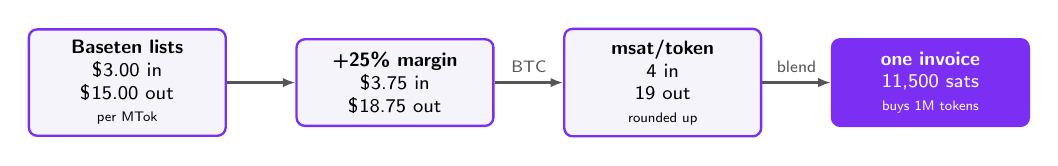
\begin{tikzpicture}[
    b/.style={rectangle, rounded corners=3pt, draw=llpurple, line width=0.85pt,
      fill=llcodebg, align=center, font=\fontsize{7.0}{8.2}\selectfont,
      minimum height=1.1cm, minimum width=2.5cm, inner sep=4pt},
    a/.style={-{Latex[length=1.6mm]}, llgraytext, line width=0.8pt},
    lbl/.style={font=\fontsize{6.0}{7}\selectfont, text=llgraytext, align=center},
  ]
    \node[b] (u) at (-5.1,0) {\textbf{Baseten lists}\\\$3.00 in\\\$15.00 out\\{\tiny per MTok}};
    \node[b] (m) at (-1.7,0) {\textbf{+25\% margin}\\\$3.75 in\\\$18.75 out};
    \node[b] (r) at (1.7,0) {\textbf{msat/token}\\4 in\\19 out\\{\tiny rounded up}};
    \node[b, fill=llpurple, text=white] (q) at (5.1,0) {\textbf{one invoice}\\11,500 sats\\{\tiny buys 1M tokens}};

    \draw[a] (u) -- (m);
    \draw[a] (m) -- node[lbl, above]{BTC} (r);
    \draw[a] (r) -- node[lbl, above]{blend} (q);
  \end{tikzpicture}
  \end{center}

  \vspace{0.2cm}
  {\footnotesize A bundle is priced at the \emph{blended} rate, the average of
  both directions. Debits are then \textbf{direction-weighted} against that
  blend, so the margin holds regardless of the buyer's prompt/completion mix,
  and rounding always goes \emph{up}, since a rate that rounds to zero is a
  free model.}

  \vspace{0.14cm}
  {\footnotesize\textbf{The honest trade-off.} Prepaid metering relaxes
  atomicity from per-request to \emph{per-bundle}: the payment is still proven
  by its preimage, but the requests drawing it down are on credit. Closing that
  gap is next.}

  \slidefooter
\end{frame}

% ----------------------------------------------------------------------------
% SLIDE 8: DEMO
% ----------------------------------------------------------------------------
\begin{frame}[plain]
  \begin{tikzpicture}[remember picture, overlay]
    \fill[llblack] (current page.south west) rectangle (current page.north east);
  \end{tikzpicture}
  \drawDecorativeSquares
  \begin{tikzpicture}[remember picture, overlay]
    \node[anchor=north west, text=white, font=\fontsize{44}{50}\selectfont\bfseries]
      at ([shift={(1.2cm,-1.7cm)}]current page.north west)
      {Demo};
    \node[anchor=north west, text=llyellowgreen, font=\Large\bfseries, text width=11.5cm]
      at ([shift={(1.2cm,-3.3cm)}]current page.north west)
      {Signet. A web wallet, an invoice, and Kimi K3.};
    \node[anchor=north west, text=llcyan, font=\normalsize, text width=11.2cm]
      at ([shift={(1.2cm,-4.5cm)}]current page.north west)
      {Kimi K3 provisioned on Baseten, \texttt{/fund} paid from the Wavelength
       web wallet, then prompt: 402, swap, preimage, stream. Close on
       \texttt{/receipts}.};
    \node[anchor=south west, text=llgraylight, font=\tiny]
      at ([shift={(0.8cm,0.4cm)}]current page.south west)
      {Every layer is real: real swap, real invoice, real preimage, real
       model, real usage debit.};
  \end{tikzpicture}
\end{frame}

% ----------------------------------------------------------------------------
% SLIDE 9: NEXT STEPS / WHERE L402 GOES
% ----------------------------------------------------------------------------
\begin{frame}[plain]
  \sectiontitle{Next: Furthering L402, Not Replacing It}
  \vspace{0.06cm}

  {\footnotesize Keep the atomic core, bring the session economics in. Every
  row below is a caveat or a rail, not a redesign.}

  \vspace{0.14cm}
  \begin{center}
  {\scriptsize
  \renewcommand{\arraystretch}{1.1}
  \begin{tabularx}{0.98\textwidth}{@{}c l X c@{}}
    \textbf{Phase} & \textbf{What} & \textbf{Why} & \textbf{Payable now?}\\
    \midrule
    0 & Session caveats + bound descriptor &
      Bundle, model, and budget become caveats over a committed JSON descriptor &
      \textcolor{llcyan}{\textbf{yes}}\\
    1 & Signed usage receipts &
      The server signs each tick, so the draw-down stops being trusted &
      \textcolor{llcyan}{\textbf{yes}}\\
    1 & Proof-of-possession caveat &
      A session pubkey, so a long-lived credential isn't a pure bearer secret &
      \textcolor{llcyan}{\textbf{yes}}\\
    2 & VHTLC deposit with a refund branch &
      Unspent balance reclaimable on timeout: real escrow, not an IOU &
      \textcolor{llorange}{\textbf{wallet work}}\\
    3 & BOLT12 payment plane &
      An offer is a stable endpoint, so top-ups leave the request path &
      \textcolor{llred}{\textbf{needs BOLT12}}\\
    \bottomrule
  \end{tabularx}}
  \end{center}

  \vspace{0.18cm}
  {\footnotesize \textbf{Phase 1 matters most:} a signed receipt chain makes a
  billing discrepancy \emph{provable} rather than a disagreement. Nearer term:
  land aperture\#247 and move to mainnet on live rates.}

  \slidefooter
\end{frame}

% ----------------------------------------------------------------------------
% SLIDE 10: CLOSE
% ----------------------------------------------------------------------------
\begin{frame}[plain]
  \begin{tikzpicture}[remember picture, overlay]
    \fill[llblack] (current page.south west) rectangle (current page.north east);
  \end{tikzpicture}
  \drawDecorativeSquares
  \begin{tikzpicture}[remember picture, overlay]
    \node[anchor=north west, text=white, font=\fontsize{30}{36}\selectfont\bfseries,
      text width=11.5cm]
      at ([shift={(1.2cm,-1.5cm)}]current page.north west)
      {Sats are enough.};
    \node[anchor=north west, text=llcyan, font=\normalsize, text width=11.2cm]
      at ([shift={(1.2cm,-2.9cm)}]current page.north west)
      {The most capable open-weights model in the world is a 1.5 TB download
       almost nobody can run, so access runs through whoever will sell you
       inference. That gate has been a credit card.};
    \node[anchor=north west, text=llyellowgreen, font=\normalsize\bfseries,
      text width=11.2cm]
      at ([shift={(1.2cm,-5.1cm)}]current page.north west)
      {It doesn't have to be. A wallet with sats, an L402 challenge, and a
       preimage get you the same tokens: no account, no key, no permission.};
    \node[anchor=south west, text=llgraylight, font=\tiny]
      at ([shift={(0.8cm,0.4cm)}]current page.south west)
      {github.com/lightninglabs/pi-402 \quad$\cdot$\quad
       \texttt{pi install git:github.com/lightninglabs/pi-402}};
  \end{tikzpicture}
\end{frame}

\end{document}
